\chapter{Evaluation}\label{chap:6}


\section{Accuracy evaluation}
As previously stated, we obtained ? malware PE file, used ? malware PE file for make $8$ decision tree. Therefore, we used ? malware meta-data as training data, in order to sort $8$ decision tree, and we make the best order of decision tree which shown in Figure \ref{fig:ordertree}, this order have the best experimental result with ? malware training data. 
Finally, malware meta-data to test experimental result our system.
With experimental result, the order of decision tree is shown in Figure \ref{fig:ordertree}.
\begin{figure}[httb]
  \centering
    
\includegraphics[width=1\textwidth]{graph/ordertree.jpg}
     \caption{The best decision tree order.}
     \label{fig:ordertree}
\end{figure}

With the order of decision tree, we use 100 malware to test the experimental result our system. In Table \ref{fig:experimentalresult}, we show the experimental result of our system. Some of number in axis show these total number of malware in that family, and that number is separated into group that these malware has been classified by our system. For example, we have 4 malware in Win32/Virut family, and we successfully classify 3 malware into Win32/Virut  family and have false to classify 1 malware into other family. Therefore, Our system also recognizes the trojan agent family with 75 \% accuracy.\\
\\

\begin{figure}[h!]
  \begin{center}
    \begin{tabular}{ | l | l | l | l | l | l | l | l | l | l |}
     \hline
    Malware & Virut & Autorun & IRCbot & Gaobot & Waledac & Downadup & Sality & Mota & Accuracy\\ \hline
    Virut & ? & ? & ? & ? & ? & ? & ? & 75\% \\ \hline
	Autorun & 0 & 0 & 0 & ? & ? & ? & ? & 50\% \\ \hline
	IRCbot & 0 & 0 & 2 & 0 & 1 & 0 & 0 & 66\% \\ \hline
	Gaobot & 1 & 0 & 0 & 2 & 8 & 0 & 3 & 53\% \\ \hline
	Waledac & 0 & 0 & 0 & 0 & 0 & 0 & 0 & 0\% \\ \hline
	Downadup & 0 & 0 & 0 & 0 & 0 & 1 & 1 & 50\% \\ \hline
	Sality & 0 & 0 & 0 & 0 & 0 & 1 & 1 & 50\% \\ \hline
	Mota & 4 & 4 & 2 & 3 & 15 & 2 & 41 & 57\% \\ \hline

    \end{tabular}
	\end{center}
     \caption{Experimental result}
    \label{fig:experimentalresult}
\end{figure} 

Our system is useful to help virus researcher determined the malware family that unknown malware belongs to. The malware family contains Win32/Virut, Win32/Autorun, Win32/IRCbot, Win32/Gaobot, Win32/Waledac, Win32/Downadup, Win32/Sality, W32.Mota, known as famous malware family. Virus research who know the family of malware can easily determined some semantic similarity between malware and showed their inner similarity in behavior and static malware characteristic.

\section{Efficiency of classifying}
Figure show comparing the step to detect semantic malware characterization using Virus total with our approach.
 \begin{figure}[httb]
  \centering
    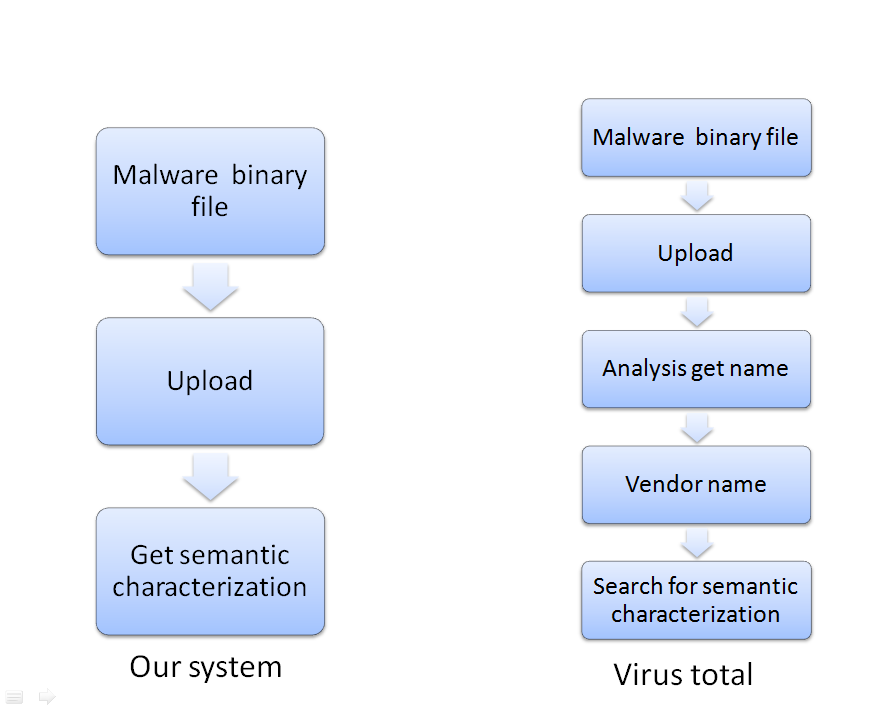
\includegraphics[width=1\textwidth]{graph/evaluation3.png}
     \caption{The best decision tree order.}
     \label{fig:evaluation3}
\end{figure}

The figure 1 show classifying time in our system. The evaluation was performed on a 2.4 HZ core i3 laptop with 4G memory, running in ubuntu 11.4. 	

\begin{figure}[httb]
  \centering
    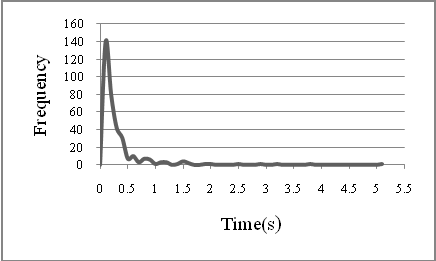
\includegraphics[width=1\textwidth]{graph/evaluation2.png}
     \caption{The best decision tree order.}
     \label{fig:evaluation2}
\end{figure}
The result was shown in figure \ref{fig:evaluation1}. The median time to perform classification was 0.25 seconds. The slowest sample classified required 5.12 seconds. Only 6 samples required more than 2 seconds. Processing time of followgraph approach was shown in figure \ref{fig:evaluation2}.

